\documentclass[11pt]{memoir}
\usepackage{amsmath}
\usepackage[polutonikogreek,francais,english]{babel}
\usepackage{setspace}
\usepackage{subfig}  
\usepackage{booktabs}
\usepackage{titlesec}
\usepackage{url}
\usepackage{graphicx} 
\usepackage{longtable}
\usepackage{makecell} 
\usepackage{bigdelim}
\usepackage{multirow}
\usepackage{caption}
\captionsetup{font=small}
\usepackage{wrapfig}
\usepackage{braket}
\usepackage{chemfig}
\usepackage{amssymb}
\usepackage{wasysym}
\usepackage[stable]{footmisc}
\usepackage{textcomp}



\usepackage{graphicx}  % provides macros for importing of graphics
%\usepackage{fullpage}  % sets margins to fill out the page (1")
\usepackage{url}       % provides easy URL formatting
\usepackage{amsmath}   % provides mathematics macros
\usepackage{setspace}  % provides macros for manipulating spacing
%\usepackage{floatflt} %
%\usepackage{fancyhdr}  % provides macros for setting running headers, etc
\usepackage{titlesec}  % provides macros for manipulating section formats
\usepackage{wrapfig}   % provides macros for figures to be wrapped by text
%\pagestyle{fancy}
 
%
% Set some global parameters
%
\settrimmedsize{11in}{210mm}{*} 
\setlength{\trimtop}{0pt} 
\setlength{\trimedge}{\stockwidth} 
\addtolength{\trimedge}{-\paperwidth} 
\settypeblocksize{7.75in}{33pc}{*} 
\setulmargins{4cm}{*}{*} 
\setlrmargins{1.25in}{*}{*} 
\setmarginnotes{17pt}{51pt}{\onelineskip} 
\setheadfoot{\onelineskip}{2\onelineskip} 
\setheaderspaces{*}{2\onelineskip}{*} 
\checkandfixthelayout 

\setcounter{secnumdepth}{0} % only the chapters will display numbers
\setcounter{tocdepth}{1}    % only chapters and section will appear in TOC
%
% define places to look for figures so that we don't have to include the directory-name every time
% we refer to a figure
%
\graphicspath{{ }{./fig/}}
%{./chapterI/fig/}{./chapterII/fig/}{./chapterIII/fig/}{./chapterIV/fig/}{./chapterV/fig/}}
%
% Define some math commands
%
\renewcommand{\vec}[1]{\mathbf{#1}}
\newcommand{\dif}[1]{\frac{d}{d #1}}
\newcommand{\Dif}[1]{\frac{\partial}{\partial #1}}
\newcommand{\der}[2]{\frac{d #2}{d #1}}
\newcommand{\Der}[2]{\frac{\partial #2}{\partial #1}}
\newcommand{\dder}[2]{\frac{d^2 #2}{d #1^2}}
\newcommand{\DDer}[2]{\frac{\partial^2 #2}{\partial #1^2}}
\newcommand{\MDer}[3]{\frac{\partial^2 #3}{\partial #1\partial #2}}
\renewcommand{\colon}{\negthinspace :\negthinspace}
\newcommand{\ratio}[2]{#1\negthinspace :\negthinspace #2}
%
% Code below defines a new enumerate environment where spacing between items can be controlled. 
% Used at end of Einstein paper.
\newenvironment{tight_enumerate}{
\begin{enumerate}
  \setlength{\itemsep}{3pt}
  \setlength{\parskip}{0pt}
}{\end{enumerate}}
% End of new enumerate environment

% abbreviations
%
\providecommand{\e}[1]{\ensuremath{\times 10^{#1}}}

\def\etal{{\textsl et al.}}
\def\ie{{\textsl i.e.}}
\def\eg{{e.g.}}
\def\th{{$^{th}$}}
\def\nd{{$^{nd}}}
\def\st{{$^{st}$}}
\def\etc{{\textsl etc.}}
 
\hyphenation{
ab-sorp-tion ac-com-pan-ied a-chieved ag-gre-gate al-ter-na-tive al-though a-nal-o-gy ap-pa-rat-us ap-pli-ca-tion ap-plied ap-pro-pri-ate ap-prox-i-ma-tion ap-prox-i-ma-tions ar-range-ment ar-range-ments as-so-ci-a-tion as-sump-tion at-ten-tion base-ment be-cause be-long be-tween Boltz-mann cal-cu-la-tion ca-ta-stro-phe char-ac-ter char-ac-ter-iz-ing char-ac-ter-is-tic char-ac-ter-ize char-ac-ter-ized chem-i-stry cir-cum-stan-ces clas-si-cal co-in-ci-dence com-bi-na-tion com-pare com-pared com-po-nents com-plete-ly com-pli-ca-ted com-pu-ta-tions con-di-tions con-nect-ed con-nec-tion con-se-quence con-se-quent con-sid-er-a-tion con-sid-ered con-stant con-stants con-struct-ing con-tra-dict cor-pus-cul-ar cor-rel-a-tive-ly cor-re-spond-ing cy-lin-dri-cal deal-ing de-lo-cal-iz-a-tion de-lo-cal-ize de-lo-cal-ized de-scrib-ing de-scrip-tion de-tec-tor de-tec-tors de-ter-mined de-vel-op-ment di-a-phragm dif-fer-end dis-ap-pear dis-ap-pears dis-crim-i-na-tion dis-place-ment dis-cus-sion dis-per-sion dis-sem-i-nates dis-tance dis-tan-ces dis-tin-guish dis-trib-ut-ed e-lec-tro-mag-net-ic e-lec-tron e-lec-trons el-e-ment el-e-men-ta-ry e-mit-ted en-er-gy en-er-gies en-tire-ly en-vi-ron-ment e-qua-tion e-qui-lib-ri-um e-qui-par-ti-tion e-ven-tu-al-i-ty ex-cep-tion-al ex-chang-es ex-ist-ence ex-pe-ri-en-ces ex-pe-ri-ence ex-per-i-ment ex-per-i-ments ex-per-i-men-tal ex-per-i-ment-al-ly ex-plains ex-pla-na-tion ex-po-nen-tial ex-po-nen-tials ex-press-es ex-treme-ly fluc-tu-a-tions fol-low-ing for-mu-lat-ed for-mu-late foun-da-tion fre-quen-cies fre-quen-cy fun-da-men-tal ge-o-met-ric-al ge-o-met-ric-al-ly grav-i-ta-tion-al guid-ing har-mon-ics Heis-en-berg ho-mo-ge-ne-ous hy-dro-gen hy-poth-e-sis im-por-tant in-can-des-cent in-com-plete in-creas-ing in-deed in-de-pen-dent in-de-ter-mi-nate in-de-ter-min-a-cy in-e-qual-i-ty in-for-ma-tion in-stru-ment in-stru-ments in-ter-ac-tion in-ter-est-ed in-ter-fer-ence in-ter-fer-om-e-ter in-ter-mo-lec-u-lar in-ter-pre-ta-tion in-tro-duc-ing in-ves-ti-gate in-volves la-bo-ra-to-ry lo-cal-ize lo-cal-ized math-e-mat-ics math-e-mat-i-cal Mau-per-tuis Max-wel-li-an me-chan-i-cal me-chan-ics mean-ing-less meas-ure-ment meas-ure-ment meas-ure-ments mol-e-cules mo-men-tum nev-er-the-less nu-mer-ous ob-jec-tion ob-jec-tions ob-ser-va-tion ob-serv-a-ble ob-serv-a-bles ob-served par-tic-u-lar par-tic-u-lar-ly par-tic-u-lars per-mit-ting per-pen-dic-u-lar phe-nom-e-na pho-to-di-ode pho-to-di-odes pho-to-e-lec-tric pho-to-graph-ic pho-to-lu-mi-nes-cence phys-i-cal phy-si-cists pol-ar-i-za-tion pol-a-rize pol-a-rized pol-a-riz-er pol-a-riz-ers pos-si-bil-i-ties pos-si-bil-i-ty po-ten-tial pre-cis-ion pre-dic-tion prin-ci-ple pro-ced-ure pro-duce pro-duced pro-per-ties pro-per-ty pro-por-tion-al pro-vid-ed quan-ti-ta-tive quan-ti-ties quan-ti-za-tion quant-um ques-tion ques-tions ra-di-a-tion re-cog-ni-tion re-pre-sen-ta-tion re-flect-ed re-gard-ing re-placed re-quest-ed ri-gid-ly Ruth-er-ford sche-mat-ic-al-ly sep-a-rate sep-a-rat-ed sim-pli-fi-ca-tion si-mul-ta-ne-ous sit-u-a-tion some-what Som-mer-feld spec-trom-e-ter spec-tro-scop-ic spec-trum stand-ard stand-ing some-thing struc-ture sub-stan-ces sub-trac-tions suc-ces-sive su-per-po-si-tion sup-posed sur-round-ing sur-round-ings tem-per-a-ture the-o-ret-i-cal ther-mal trans-mit-ted treat-ment un-der-stand-ing Thom-son un-a-void-a-bly un-der-stand-a-ble un-found-ed Un-ge-nau-ig-keit-en un-pre-dict-a-ble var-i-a-ble 
}




%% DRS: This allows us to manually specify header content. See Morgan chapter for more deatils.
\pagestyle{myheadings}

%% DRS: This redefines how figures are labeled (no chapter number)
%\renewcommand{\thefigure}{\arabic{figure}}

%
% Above replaced with manual figure numbers throughout
% using \caption*{}
%

\chapterstyle{thatcher}
\renewcommand{\chaptitlefont}{\normalfont\scshape\huge}

\renewcommand{\prechapterprecis}{%
  \vspace*{\prechapterprecisshift}%
  \begin{center}\precisfont}
\renewcommand{\postchapterprecis}{\end{center}}
\renewcommand*{\precisfont}{\normalfont\scshape}

%% DRS: The following commands change the font families for the entire document. I chose Palatino. See the supporting docs for more info on font choices.
\renewcommand{\rmdefault}{ppl}
\renewcommand{\sfdefault}{phv}
\renewcommand{\ttdefault}{pcr}
\usepackage[left=1.5in,right=1in,top=1in,bottom=1.0in]{geometry} 
 


% Acknowledgments page: also note the conventions (bracketed footnotes, asterisks for ellipsis,
% block quotes for original papers interspersed with commentary [name chapters])

\begin{document}

\setlength{\aboverulesep}{0pt} % from {booktabs} for better rules in tables
\setlength{\belowrulesep}{0pt}
  
\titleformat{\section}{\normalfont\Large\scshape\centering}{\thesection}{}{}
\titleformat{\subsection}{\normalfont\bfseries}{\thesubsection}{}{}



\frontmatter

\mainmatter
\pagenumbering{arabic}

%\chapter{The Atom and the Molecule}

\thispagestyle{plain}

\begin{center}
	{\LARGE THE ATOM AND THE MOLECULE}
\end{center}

\chapterprecis{Gilbert N. Lewis\footnote{Received January 26, 1916. Reprinted from the \emph{Journal of the American Chemical Society}, Vol. XXXVIII. No. 4. April, 1916.}} 

\makeoddhead{myheadings}{\emph{Lewis}}{}{\thepage}
\makeevenhead{myheadings}{\thepage}{}{\emph{The Atom and the Molecule}}
 
In a paper entitled ''Valence and Tautomerism''\footnote{\textbf{\textsc{This Journal}, 35}, 1448, (1913); see also the important article of Bray and Branch, \emph{Ibid.,} \textbf{35}, 1440 (1913).} I took occasion to point out the great importance of substituting for the conventional classification of chemical substances, as inorganic or organic, the more general classification which distinguishes between polar and nonpolar substances.  The two classifications roughly coincide, since most inorganic substances are distinctly polar, while the majority of organic substances belong to the nonpolar class; thus potassium chloride represents the extreme polar type and methane the nonpolar.  Nevertheless, there are many inorganic substances which, under ordinary circumstances, are predominantly nonpolar, and many organic substances which, at least in a certain part of the molecule, are strongly polar.

This article was apparently unknown to Sir. J. J. Thomson\footnote{\emph{Phil. Mag.}, \textbf{27}, 757 (1914).} when he wrote, in 1914, an extremely interesting paper on the ''Forces between Atoms and Chemical Affinity'' in which he reached conclusions in striking accord with my own, and discussed in considerable detail the theories of atomic and molecular structure which led him to these conclusions.

To enable us to appreciate the importance and the usefulness of a distinction between the polar and nonpolar types of chemical molecules no hypotheses are necessary, but in a more minute examination of the nature of such a distinction some theory of atomic structure is indispensable.  Such a theory I have employed for a number of years in the interpretation of chemical phenomena, but it has not hitherto been published.  I shall present this theory briefly in the present paper, for, while it bears much resemblance to some current theories of the atom, it shows some radical points of departure from them.  As an introduction it will be desirable to review the characteristics of polar and nonpolar compounds.

\section*{Polar and Nonpolar Types}

The very striking differences in properties between the extreme polar and the extreme nonpolar types are summarized in the following table quoted from my previous paper:\footnote{In my former paper the words ''inert'' and ''reactive'' were inadvertently transposed and appear in the wrong columns. [See second row of chart.]}

% Polar Nonpolar Table
\begin{center}
\begin{tabular}{ l l }
	POLAR &  NONPOLAR \\ 
	  & \\
	Mobile & Immobile \\ 
	Reactive & Inert  \\
	Condensed structure & Frame Structure \\
	Tautomerism & Isomerism  \\
	Electrophiles & Non-electrophiles \\
	Ionized & Not ionized \\
	Ionizing solvents & Not ionizing solvents \\
	High dielectric constant & Low dielectric constant \\
	Molecular complexes & No molecular complexes \\
	Association & No association \\
	Abnormal liquids & Normal liquids \\
	
\end{tabular} \vspace{5mm}
\end{center}

All of these properties with respect to which fundamental distinctions have been made between the two types, and which seem so unconnected, are in fact closely related, and the differences are all due to a single cause.  Even before making any more special hypothesis we may very safely assume that the essential difference between the polar and the nonpolar molecule is that, in the former, one or more electrons are held by sufficiently weak constraints so that they may become separated from their former positions in the atom, and in the extreme case pass altogether to another atom, thus producing in the molecule a bipole or multipole of high electrical moment.  Thus in an extremely polar molecule, such as that of sodium chloride, it is probable that at least in the great majority of molecules the chlorine atom has acquired a unit negative charge and therefore the sodium atom a unit positive charge, and that the process of ionization consists only in a further separation of these charged parts.

If then we consider the nonpolar molecule as one in which the electrons belonging to the individual atom are held by such constraints that they do not move far from their normal positions, while in the polar molecule the electrons, being more mobile, so move as to separate the molecule into positive and negative parts, then all the distinguishing properties of the two types of compounds become necessary consequences of this assumption, as we may readily show.

Thus polar compounds with their mobile parts fall readily into those combinations which represent the very few stable states, while the nonpolar molecules, in which the parts are held by firmer constraints, are inert and unreactive, and can therefore be built up into the numerous complicated structures of organic chemistry.  Many organic compounds, especially those containing elements like oxygen and nitrogen and those which are said to be unsaturated, show at least in some part of the molecule a decidedly polar character.  In such cases we have the phenomenon of tautomerism, where two or more forms of the molecule pass readily into one another and exist together in a condition of mobile equilibrium.  Tautomerism is not characteristic of organic substances, but is, on the other hand, a predominant trait of most inorganic substances, which behave as if a great variety of forms were existing together in extremely mobile equilibrium.

When a molecule owing to the displacement of an electron, or electrons, becomes a bipole (or multipole) of high electrical moment, that is, when its charged parts are separated by an appreciable distance, its force of attraction for another molecular bipole will be felt over a considerable intervening distance, and two or more such bipoles will frequently be drawn together into a single aggregate in which the positive part of one molecule is brought as near as possible to the negative part of another.  The molecules of a polar substance will therefore not only exhibit an unusually high intermolecular attraction at a distance, but will frequently combine with one another and show the phenomenon known as association.  It is indeed the substances which are distinctly polar, like ammonia, water, acids, and alcohols, which constitute, on account of association as well as of high intermolecular attraction, a class of liquids which are called abnormal with respect to numerous properties such as critical point, vapor pressure, heat of vaporization, viscosity, and surface tension.

Moreover a polar substance will combine with other substances to form those aggregates which are sometimes known as molecular compounds or complexes, and it may so combine with substances which are not of themselves markedly polar, for in the presence of a polar substance all other substances become more polar.

This important effect of polar molecules in rendering others more polar, to which I called attention in my previous paper, has been discussed in some detail by Thomson.  A molecular bipole of small molecular moment, which would scarcely attract a similar molecule, will be very appreciably attracted by a polar molecule or bipole of high moment, and may form with it a double molecule.  In this process the weaker bipole stretches and its moment increases.  In general, if two molecules combine or even approach one another, each weakens the constraints which hold together the charge of the other, and the electrical moment of each is increased.

This increase in the polar character of a molecule when combined with, or in the neighborhood of, other polar molecules is to a remarkable degree cumulative, for when two molecules by their approach or combination become more polar they draw other molecules more strongly towards them, but this still further increases their polar character.  This is strikingly illustrated in numerous phenomena.  Thus two substances in the gaseous state may differ but little in polar character, but when they are condensed to liquids the differences are frequently enormous.

\renewcommand{\thefigure}{\arabic{figure}}
\setcounter{figure}{0}

\begin{figure}
	\begin{center}
		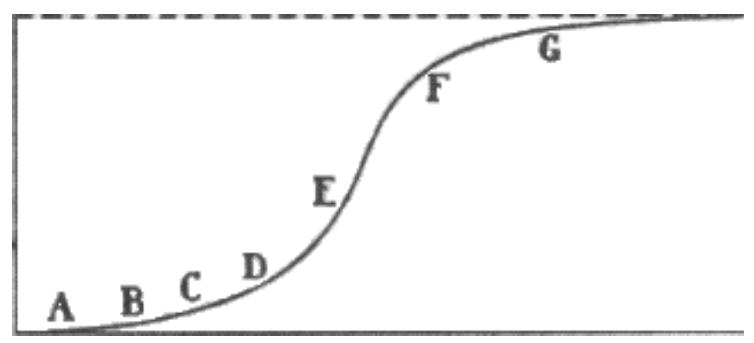
\includegraphics[width=0.6\textwidth]{images/lewis_figure1.png}
	\end{center}
	% Use the following command to remove the colon from the figure label; Always use it within the environment to keep it local
%%%%	\makeatletter \renewcommand{\fnum@figure}[1]{\figurename~\thefigure} \makeatother
	\caption*{Figure 1}

       % \label{fig:figureX}

%\vspace{-10pt}
\end{figure}



The polar character of a substance depends, therefore, not only upon the specific properties of the individual molecules, but also upon what we may call the strength of the polar environment.  Without attempting to give any quantitative definition of our terms we may plot, as in Figure 1, the degree of polarity of a substance as ordinate and the strength of the polar environment as abscissa.  We then have for all substances a curve of the type shown in the figure where the dotted line represent the highest degree of polarity, namely complete ionization.  Different pure substances in the liquid state come at different points, thus, roughly, hexane at $A$; benzene at $B$; ether at $C$; esters at $D$; water, ammonia, alcohols, amines, acids between $D$ and $F$; and fused salts at $G$.  In the last case, since the substance has nearly reached its highest possible polarity, it will not be much affected by an increase in the strength of the polar environment.  At the other end of the curve a substance at $A$ in a strong polar environment may move to $B$, and one at $B$ may move to $C$, but they would not become markedly polar.  It is in the intermediate range that substances are most affected by small changes in the environment.  Thus hydrochloric acid, which in the pure state is not extremely polar, reaches nearly the highest possible state of polarity when dissolved in water.  Such a change in this region is often much accentuated by the formation of complexes, and thus we have the rule of Abegg and Bodl\"{a}nder that a weak electrolyte usually becomes a strong electrolyte when its weak ion is converted into a complex ion.

We come then to the consideration of the electrical properties which distinguish polar from nonpolar substances, or, in accordance with the terminology which I formerly used,\footnote{Lewis and Wheeler, \emph{Z. physik. Chem.}, \textbf{56}, 189 (1906).} which distinguish good electrophiles from poor electrophiles.

The first difference is in the dielectric constant.  The difference between the dielectric constant of a substance and that of free space measures directly the number of free charges in the substance multiplied by the average distance through which these charges move under the influence of a definite electric field.  In the polar molecule the constraints which operate against a separation of the charges, begin already weak, may be further stretched in the electric field, and what is more important, the bipoles (or multipoles) which already exist in the polar substance may, by rotation, orient themselves in the electric field, thus producing a large displacement current and therefore a high dielectric constant.  In this connection Thomson has called attention to the work of Baedeker,\footnote{\emph{Z. physik. Chem.}, \textbf{36}, 305 (1901).} which shows that even in the gaseous state such substances as ammonia, water and hydrochloric acid possess an abnormally high dielectric constant.

Finally the polar substance, whether in the pure state or dissolved in another solvent, will obviously be one which will be readily ionized.  Moreover, polar substances are the strong ionizing solvents, for when another substance is combined with a highly polar substance, or even dissolved in such a solvent without actual combination of molecules, the degree of its own polarity largely increases.

Wide apart as the polar and nonpolar types are in the extreme, we must nevertheless inquire whether the difference is one of kind or one of degree. If there were a sharp and always recognizable distinction between the polar and the nonpolar molecule then a substance would be more polar or less polar according as it possessed a greater or smaller percentage of molecules of the first type.  This would be a simple and in many cases a satisfactory interpretation of the difference in behavior between different substances, but scanning the whole field of chemical phenomena we are, I believe, forced to the conclusion that the distinction between the most extreme polar and nonpolar types is only one of degree, and that a single molecule, or even a part of a molecule, may pass from one extreme type to another, not by a sudden and discontinuous change, but by imperceptible gradations.  The nature of such a transition we shall discuss in the following sections:

\section*{The Cubical Atom.}

A number of years ago, to account for the striking fact which has become known as Abegg's law of valence and countervalence, and according to which the total difference between the maximum negative and positive valences or polar numbers of an element is frequently eight and is in no case more than eight, I designed what may be called the theory of the cubicle atom.  This theory, while it has become familiar to a number of my colleagues, has never been published, partly because it was in many respects incomplete.  Although many of these elements of incompleteness remain, and although the theory lacks today much of the novelty which it originally possessed, it seems to me more probable intrinsically than some of the other theories of atomic structure which have been proposed, and I cannot discuss more fully the nature of the differences between polar and nonpolar compounds without a brief discussion of this theory.

\begin{figure}
	\begin{center}
		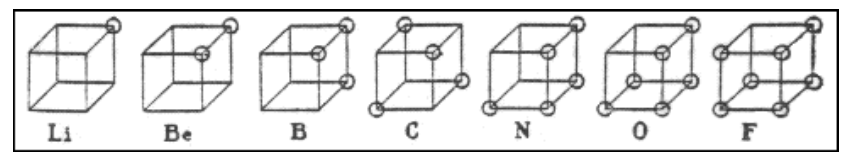
\includegraphics[width=0.6\textwidth]{images/lewis_figure2.png}
	\end{center}
	% Use the following command to remove the colon from the figure label; Always use it within the environment to keep it local
%%%%	\makeatletter \renewcommand{\fnum@figure}[1]{\figurename~\thefigure} \makeatother
	\caption*{Figure 2}

       % \label{fig:figureX}

%\vspace{-10pt}
\end{figure}


%Fig.2
The pictures of atomic structure which are reproduced in Figure 2,\footnote{These figures are taken from a memorandum dated March 28, 1902, together with the models are notes concerning different types of chemical compounds; the various possible arrangements of electrons in the outer atom and the possibility of intra-atomic isomerism; the relationship between symmetrical structure and atomic volume; and certain speculations as to the structure of the helium atom which we shall see were probably partly incorrect.  The date of origin of this theory is mentioned not with the purpose of claiming any sort of priority with respect to those portions which overlap existing theories but because the fact that similar theories have been developed independently adds to the probability that all possess some characteristics of fundamental reality.} and in which the circles represent the electrons in the outer shell of the neutral atom, were designed to explain a number of important laws of chemical behavior with the aid of the following postulates:

\begin{enumerate}
\item In every atom is an essential \emph{kernel} which remains unaltered in all ordinary chemical changes and which possesses an excess of positive charges corresponding in number to the ordinal number of the group in the periodic table to which the element belongs.
\item The atom is composed of the kernel and an \emph{outer atom or shell}, which, in the case of the neutral atom, contains negative electrons equal in number to the excess of positive charges of the kernel, but the number of electrons in the shell may vary during chemical change between 0 and 8.
\item The atom tends to hold an even number of electrons in the shell, and especially to hold eight electrons which are normally arranged symmetrically at the eight corners of a cube.\footnote{We shall see later the advisability of modifying this assumption of the cubic arrangement of the fundamental group of eight electrons.}
\item Two atomic shells are mutually interpenetrable.
\item Electrons may ordinarily pass with readiness from one position in the outer shell to another.  Nevertheless they are held in position by more or less rigid constraints, and positions and the magnitude of the constraints are determined by the nature of the atom and of such other atoms as are combined with it.
\item Electric forces between particles which are very close together do not obey the simple law of inverse squares which holds at greater distances.
\end{enumerate}

Some further discussion of these postulates is necessary in order to make their meaning clear.  The first postulate deals with the two parts of the Thomson atom.  The kernel being that part of the atom which is unaltered by ordinary chemical change is of sufficient importance to merit a separate symbol.  I propose that the common symbol of the element will stand for the lithium kernel.  It has a single positive charge and is equivalent to pure lithium ion $Li^+$.  \textbf{Be} has two positive charges, \textbf {B} three, \textbf{C} four, \textbf{N} five, \textbf{O} six, and \textbf{F} seven.

We might expect the next element in the series, neon, to have an atomic kernel with eight positive charges and an outer shell consisting of eight electrons.  In a certain sense this is doubtless the case.  However, as has been stated in Postulate 3, a group of eight electrons in the shell is extremely stable, and this stability is the greater the smaller the difference in charge between the nucleus and this group of eight electrons.  Thus in fluoride ion the kernel has a charge of +7, and the negative charge of the group of eight electrons only exceeds it by one unit.  In fact in compounds of fluorine with all other elements, fluorine is assigned the polar number -1.  In the case of oxygen, where the group of eight electrons has a charge exceeding that of the kernel by two units, the polar number is considered to be -2 in nearly every compound.  Nitrogen is commonly assumed to have the polar number -3 in such compounds as ammonia and the nitrides.  It may be convenient to assign occasionally to carbon the polar number -4, but it has never been found necessary to give boron a polar number -5, or beryllium -6, or lithium -7.  But neon, with an inner positive charge of 8 and an outer group of eight electrons, is so extremely stable that it may, as a whole, be regarded as the kernel of neon and we may write \textbf{Ne} = Ne.\footnote{It must not be assumed, even in the case of the elements here chosen for discussion, that the distinction between kernel and shell is absolutely hard and fast.  Thus in the ionization of neon by electric discharge, electrons must be thrown off from the group which we consider as belonging to the kernel itself.}

The next element, sodium, begins a new outer shell\footnote{The periodicity in the table of elements, due to successive additions of groups of eight electrons to the atomic kernel, is imitated closely by compounds.  Thus ammonium ion has nine positive charges in the kernels and eight electrons in the shells, but these eight electrons forming a stable group make ammonium ion entirely analogous to the kernel of an alkali metal.} and \textbf{Na} = $\mathrm{Na^+}$, \textbf{Mg} = $\mathrm{Mg^{++}}$, and so on.  In my original theory I considered the elements in the periodic table thus built up, as if block by block, forming concentric cubes.  Thus potassium would be like sodium except that it would have one more cube in the kernel.  This idea, as we shall see, will have to be modified, but nevertheless it gives a concrete picture to illustrate the theory.

We have then as kernels\footnote{I believe that it will be easily remembered that the sodium kernel has one positive charge, that of chlorine seven positive charges, etc.; but it may occasionally be desirable for pedagogical purposes to attach to the symbol of the atomic kernel, a small numeral as an index, to show the number of charges.} with a single positive charge \textbf{H, Li, Na, K, Rb, Cs}; with two positive charges \textbf{Be, Mg, Ca, Sr, Ba}; with three charges \textbf{B, Al, Sc}; with four charges \textbf{C, Si}; with five charges \textbf{N, P, As, Sb, Bi}; with six charges \textbf{O, S, Se, Te} and a group of radioactive isotopes; with seven charges \textbf{F, Cl, Br, I}; and with zero charge \textbf{He, Ne, A, Kr, Xe} and \textbf{Nt}.  These elements only will be discussed in the present paper.  The remaining elements form a class in which the atomic kernel is probably neither uniquely determined nor invariable during chemical change.  This is one of the elements of incompleteness in the theory.  Nevertheless this classification is not arbitrary but is forced upon us, and the elements which are included furnish so large a part of the material upon which the science of chemistry is based, that the study of their compounds offers in itself a problem of great importance.

Postulate 2 cannot be fully discussed except in connection with the fourth postulate, but assuming that we understand the meaning of the reduction or oxidation of an element (at least in the case of highly polar substances), reduction means an increase and oxidation a decrease in the number of electrons in the outer atom of the element.  Thus for illustration, and with such reservations as will presently be shown necessary, we may state that chlorine has eight electrons in the outer shell in chlorides, six in hypochlorites, four in chlorites, two in chlorates and none in perchlorates.

Postulate 3 can best be illustrated by the use of formulae in which the electrons of the atomic shells are themselves considered as atoms of the element electricity\footnote{Dr. Branch has kindly called my attention to a little book by Sir William Ramsay (''The Temple Primers; Modern Chemistry'') in which he uses very similar formulae containing \textbf{E}.} with the symbol \textbf{E}.  Just as with ordinary symbols we use two types of formulae, one the gross formula representing hardly more than the chemical composition of the substance, the other a structural formula in which we attempt to represent the relative positions of the atoms, so we may, with the new symbols, employ the two types of formulae.  We shall later discuss the structural formula, but at this point we may consider the gross formula involving the atomic kernels and the electrons of the outer atoms.  Lithium has one positive charge in the kernel, fluorine has seven such charges, so that the neutral molecule of lithium fluoride we may represent $\mathbf{LiFE_8}$. In lithium sulfate \textbf{S} and \textbf{O} each has six positive charges and $\mathrm{Li_{2}SO_4}$ = $\mathbf{Li_2SO_4E_{32}}$; $\mathrm{SO^{--}}$ = $\mathbf{SO_4E_{32}}$.  In every substance in which each element has either its highest or its lowest polar number, \textbf{E} will appear in multiples of 8.  Thus $\mathrm{NH_3}$ = $\mathbf{NH_3E_8}$, $\mathrm{H_2O}$ = $\mathbf{H_2OE_8}$, $\mathrm{KOH}$ = $\mathbf{KOHE_8}$, $\mathrm{NaNO_3}$ = $\mathbf{NaNO_3E_{24}}$, $\mathrm{AlO_3H_3}$ = $\mathbf{AlO_3H_3E_{24}}$, $\mathrm{MgCl_2}$ = $\mathbf{MgCl_2E_{16}}$, $\mathrm{K_2CO_3}$ = $\mathbf{K_2CO_3E_{24}}$.  In compounds in which the elements have polar numbers intermediate between the highest and the lowest the number of electrons is not as a rule a multiple of 8, but is in almost all cases \emph{an even number}.  Thus $\mathrm{SO_2}$ = $\mathbf{SO_2E_{18}}$, $\mathrm{NaClO}$ = $\mathbf{NaClOE_{14}}$, $\mathrm{C_2H_2}$ = $\mathbf{C_2H_2E_{10}}$, $\mathrm{C_6H_6O}$ = $\mathbf{C_6H_6OE_{36}}$.

The extraordinary generality of this rule is shown by the fact that among the tens of thousands of known compounds of the elements under consideration only a few exceptions are known.  I may state here all of such compounds that are known to me as they form a very interesting class of substances with an even number of electrons.  First may be mentioned some of the elements themselves in the monatomic state, and as types we may take $\mathrm{Na}$ = $\mathbf{NaE}$ and $\mathrm{I}$ = $\mathbf{IE_7}$  In addition to these,\footnote{Possibly hypophosphoric acid is to be added to this list, but the evidence concerning its molecular weight does not seem conclusive.} we have $\mathrm{NO}$ = $\mathbf{NOE_{11}}$, $\mathrm{NO_2}$ = $\mathbf{NO_2E_{17}}$, $\mathrm{ClO_2}$ = $\mathbf{ClO_2E_{19}}$, $\mathrm{(C_6H_5)_3C}$ = $\mathbf{(C_6H_5)_3CE_{91}}$, as well as other tri-aryl methyls\footnote{See the review by Gombert, \textbf{This Journal, 36}, 1144 (1914).} and probably also the intensely colored compounds between metals and di-aryl ketones,\footnote{Schlenk and Weickel, \emph{Ber.}, \textbf{44}, 1182 (1914).} and the colored substances which Wieland believes to contain bivalent and quadrivalent nitrogen.\footnote{Wieland, \emph{Ann.}, \textbf{381}, 200 (1911; \emph{Ber.}, \textbf{47}, 2111, (1914).}

It is to be particularly noted that such substances when placed in a polar environment almost invariably change into substances with an even number of electrons in the outer atoms.  Thus $\mathrm{NO_2}$ dissolved in water gives nitrous and nitric acids, and even in pure liquid nitrogen tetroxide we must assume, since it has electrical conductivity, that such ions as $\mathrm{NO_2^+}$ = $\mathbf{NO_2E_{16}}$ and $\mathrm{NO_2^-}$ = $\mathbf{NO_2E_{18}}$ are present.  Similarly, $\mathrm{ClO_2}$ dissolves to form chlorous and chloric acids to a small extent, triphenyl methyl dissolves in liquid sulfur dioxide to form a conducting solution with ions presumably of the type $\mathrm{(C_6H_5)_3C^+}$ and $\mathrm{(C_6H_5)_3C^-}$.  Sodium in the metallic state, or when dissolved in such a solvent as liquid ammonia, dissociates according to the equation $\mathbf{NaE}$ = $\mathbf{Na}$ + $\mathbf{E}$.  In general, therefore, we may state that a substance, in whose gross formula an odd number of electrons appears, holds one electron by weak constraints, and in a medium which weakens all electric constraints, namely in a polar medium, the odd electron may be given up completely.  Of the cases mentioned, the odd electron appears to be most firmly bound in $\mathrm{NO}$, and even in a polar environment the constraints are still sufficiently powerful to hold the electron, that is, in the presence of a substance which has a strong tendency to take up an electron, the interchange will occur at once.

Molecules of this class which contain an odd or unpaired electron will for the sake of brevity be called \emph{odd} molecules.  An odd molecules will contain at least one atom with an uneven number of electrons in the shell.  This may be called an \emph{odd} atom.

Postulate 4 raises a question of the very greatest importance.  Ever since the first suggestion of Helmholtz, numerous efforts have been made to explain chemical combination by the assumption that in the formation of a compound some of the electrons of one atom pass completely into another atom, and that the different charged parts of the molecule thus produced are held together by electrical forces.  Such theories have in my opinion, proved entirely inadequate except in the case of substances of the strongly polar type.  This fact has been recognized by Thomson in his latest paper, in which he introduces an entirely different type of chemical combination in the case of the compounds which we have called nonpolar.  However, according to the theory which I am now presenting, it is not necessary to consider the two extreme types of chemical combination, corresponding to the very polar and the very nonpolar compounds, as different in kind, but only as different in degree.  This is due to the assumption of the interpenetrability of the atomic shells which is made in Postulate 4.  Thus an electron may form a part of the shell of two different atoms and cannot be said to belong to either one exclusively.  Hence in general it is impossible to say that one element in a compound has, during chemical change, been oxidized or reduced and that another element has not suffered such a change; but it is only as we approach substances of the completely polar type that such distinctions become less and less ambiguous.  Since this question is one to which we shall frequently revert it need not be discussed further at this point.

Postulate 5 is based upon the fact that we do not find what might be called intra-atomic isomers.  If the electrons of the atomic shell could at one time occupy one set of positions and at another time another set, and if there were no opportunity for ready transition from one of these sets of positions to another, we should have a large number of isomers differing from one another only in the situation of the electrons in the atomic shell.  While there may possibly be a few cases where we might surmise the existence of just such isomers, in most cases it is evident that they do not exist, and we must assume, therefore, considerable freedom of change from one distribution of electrons in the shell to another.

Now there are only two ways in which one body can be held by another.  It may, owing to a force of attraction, be drawn toward the second body until this force is gradually offset by a more rapidly increasing force of repulsion.  In this case it comes to rest at a point where the net attraction or repulsion is zero, and is therefore in a condition of constraint with respect to any motion along the line joining the two centers; for if the distance between the two bodies is diminished they repel one another.  An example of this type is a body attracted toward the earth but resting upon an elastic substance where the attractive force of gravity is offset by the repulsive force which we happen to call elastic; but it would be a mistake to consider the forces of elasticity to be different in character from other known forces.  Indeed it is evident that just as we have the law of universal attraction between particles at great distances, so \emph{at small distances} we have the equally universal \emph{law of repulsion}.

The other way in which one body may hold another is that in which the planets are held by the sun, and this is the way that in some current theories of atomic structure the electrons are supposed to be held by the atom.  Such an assumption seems inadequate to explain even the simplest chemical properties of the atom, and I imagine it has been introduced only for the sake of maintaining the laws of electromagnetics which are known to be valid at large distances.  The fact is, however, that in the more prominent of these theories even this questionable advantage disappears, for the common laws of electricity are not preserved.  The most interesting and suggestive of these theories is the one proposed by Bohr\footnote{I believe that there is one part of Bohr's theory for which the assumption of the orbital electron is not necessary, since it may be translated directly into the terms of the present theory.  He explains the spectral series of hydrogen by assuming that an electron can move freely in any one of a series of orbits in which the velocities differ by steps, these steps being simply expressed in terms of ultimate units (in his theory Planck's \emph{h} is such a unit), and that radiation occurs when the electron passes from one orbital velocity to the next.  It seems to me far simpler to assume that an electron may be held in the atom in stable equilibrium in a series of different positions, each of which having definite constraints, corresponds to a definite frequency of the electron, the intervals between the constraints in successive positions being simply expressible in terms of ultimate rational units (see Lewis and Adams, \emph{Phys. Rev.} \textbf{3}, 92 (1914).} and based upon Planck's quantum theory.  Plank in his elementary oscillator which maintains its motion at the absolute zero, and Bohr in his electron moving in a fixed orbit, have invented systems containing electrons of which the motion produces no effect upon external charges.  Now this is not only inconsistent with the accepted laws of electromagnetics but, I may add, is logically objectionable, for that state of motion which produces no physical effect whatsoever may better be called a state of rest.

Indeed it seems hardly likely that much progress can be made in the solution of the difficult problems relating to chemical combination by assigning in advance definite laws of force between the positive and negative constituents of an atom, and then on the basis of these laws building up mechanical models of the atom.  We must first of all, from a study of chemical phenomena, learn the structure and the arrangement of the atoms, and if we find it necessary to alter the law of force acting between charged particles at small distances, even to the extent of changing the sign of that force, it will not be the first time in the history of science that an increase in the range of observational material has required a modification of generalizations based upon a smaller field of observation.  Indeed in the present case, entirely aside from any chemical reasons, a study of the mathematical theory of the electron leads, I believe, irresistibly to the conclusion that Coulomb's law of inverse squares must fail at small distances.

In this connection I wish to call attention to an extremely interesting paper by Mr. A. L. Parson\footnote{A ''Magneton Theory of the Structure of the Atom,'' \emph{Smithsonian Publication} 2371, Washington, 1915.} which has only just been published, but which I had an opportunity of looking over with the author over a year ago.  The fundamental assumption of Parson's theory is that the electron is not merely an electric charge but is also a small magnet, or, in his terminology, a magneton.  Assuming therefore the existence of magnetic as well as electric forces between the different parts of the atom, Parson was led entirely independently to the conclusion which I have stated above, namely that the most stable condition for the atomic shell is the one in which eight electrons are held at the corners of a cube.  Not only in this but in a number of other important points the theory which I am presenting will be seen to coincide with that of Parson's paper.  The results of the magnetic experiments with which he proposes to test the magneton theory will be of great interest.  Meanwhile we may attempt to find, apart from any \emph{a priori} consideration, just what atomic structure best explains known chemical facts.

There is one part of Parson's theory which agrees with my own former theory but which I now believe to be incorrect.  The idea that argon is a system of concentric cubes (in Parson's theory cubes side by side), and that neon is a similar system with one less cube, led naturally to the assumption that helium is similarly constituted.  But recent evidence from radioactive phenomena, and from Moseley's study of the X-ray spectrum, makes it seem almost certain that helium has a total not of eight but of either two or four electrons.\footnote{Two, if hydrogen and helium are the only elements of lower atomic weight than lithium; four, if we assume with Rydberg that there are two rows in the periodic table, one containing hydrogen and proto-helium and one containing eka-hydrogen and helium.  The above discussion will be the same on either of these assumptions, and although Rydberg's assumption has a very high degree of plausibility I have adopted for simplicity the more familiar one.}  Assuming that helium is the only element between hydrogen and lithium and that it has two electrons, then it is evident from the inert character of helium, and from the resemblance of this element to the other inert gases, that here the pair of electrons plays the same role as the group of eight in the heavier atoms, and that in the row of the periodic table comprising hydrogen and helium we have in place of the rule of eight the rule of two.  Therefore hydrogen not only has one electron in its outer shell, which may pass into the shell of another atom just as the electron of lithium or sodium may, but it is capable of taking up one electron to form the stable pair, just as fluorine or chlorine takes up one electron to form the stable group of eight.  Hydrogen therefore must be regarded as the first member of the halogens as well as of the lithium group.  According to this view lithium hydride is a salt\footnote{In order to test this view experiments have been begun by Professor O. F. Stafford.  These experiments have not progressed far but they at least indicate that fused lithium hydride is a good electrolyte.} although perhaps less polar than lithium fluoride or chloride.  Therefore in what follows we shall regard the acquisition of one additional electron by hydrogen as entirely analogous to the acquisition of enough electrons to form the group of eight in the case of other atoms.

\section*{Molecular Structure.}

I shall now attempt to show how, by a single type of chemical combination, we may explain the widely varying phenomena of chemical change.  With the original assumption of Helmholtz, which has been used by some authors under the name of the electron theory of valence, according to which a given electron either does or does not pass completely from one atom to another, it is possible to give a very satisfactory explanation of compounds which are of distinctly polar type, but the method becomes less and less satisfactory as we approach the nonpolar type.  Great as the difference is between the typical polar and nonpolar substances, we may show how a single molecule may, according to its environment, pass from the extreme polar to the extreme nonpolar form, not \emph{per saltum}, but by imperceptible gradations, as soon as we admit that an electron may be the common property of two atomic shells.

Let us consider first the very polar compounds.  Here we find elements with but few electrons in their shells tending to give up these electrons altogether to form positive ions, and elements which already possess a number of electrons tending to increase this number to form the group of eight.  Thus $\mathrm{Na^+}$ and $\mathrm{Ca^{++}}$ are kernels without a shell, while chloride ion, sulfide ion, nitride ion (as in fused nitrides) may each be represented by an atom having in the shell eight electrons at the corners of a cube.


\begin{figure}
	\begin{center}
		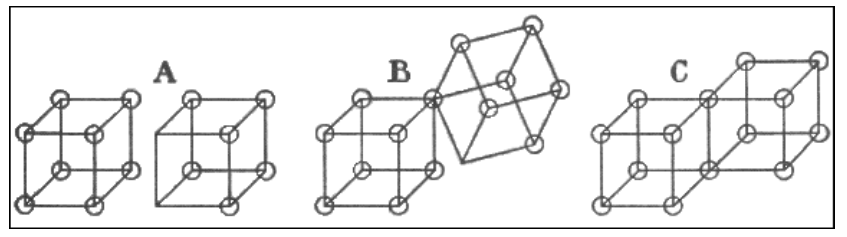
\includegraphics[width=0.6\textwidth]{images/lewis_figure3.png}
	\end{center}
	% Use the following command to remove the colon from the figure label; Always use it within the environment to keep it local
%%%%	\makeatletter \renewcommand{\fnum@figure}[1]{\figurename~\thefigure} \makeatother
	\caption*{Figure 3}

      %  \label{fig:figureX}

%\vspace{-10pt}
\end{figure}


%Fig.3
As an introduction to the study of substances of slightly polar type we may consider the halogens.  In Figure 3 I have attempted to show the different forms of the iodine molecule $\mathrm{I_2}$.  $A$ represents the molecule as completely ionized, as it undoubtedly is to a measurable extent in liquid iodine.\footnote{See Lewis and Wheeler, \emph{Loc. cit.}}  Without ionization we may still have one of the electrons of one atom fitting into the outer shell of the second atom, thus completing its group of eight as in $B$.  But at the same time an electron of the second atom may fit into the shell of the first, thus satisfying both groups of eight and giving the form $C$ which is the predominant and characteristic structure of the halogens.  Now, notwithstanding the symmetry of the form $C$, if the two atoms are for any reason tending to separate, the two common electrons may cling more firmly sometimes to one of the atoms, sometimes to the other, thus producing some dissymmetry in the molecule as a whole, and one atom will have a slight excess of positive charge, the other of negative.  This separation of the charges and the consequent increase in the polar character of the molecule will increase as the atoms become separated to a greater distance until complete ionization results.\footnote{When the separation occurs in a nonpolar environment the atoms may separate in such a way that each retains one of the two common electrons, as in the thermal dissociation of iodine gas.}  Thus between the perfectly symmetrical and nonpolar molecule $C$ and the completely polar and ionized molecule represented by $A$ there will be an infinity of positions representing a greater or lesser degree of polarity.  Now in a substance like liquid iodine it must not be assumed that all of the molecules are in the same state, but rather that some are highly polar, some almost nonpolar, and others represent all gradations between the two.  When we find that iodine in different environments shows different degrees of polarity, it means merely that in one medium there is a larger percentage of the more polar forms.  So bromine, although represented by an entirely similar formula, is less polar than iodine.  In other words, in the average molecule the separation of the charge is less than in the case of iodine.  Chlorine and fluorine are less polar than either and can be regarded as composed almost completely of molecules of the form $C$.

I wish to emphasize once more the meaning that must be ascribed to the term tautomerism.  In the simplest case where we deal with a single tautomeric change we speak of the two tautomers and sometimes write definite formulae to express the two.  But we must not assume that all of the molecules of the substance possess either one structure or the other, but rather that these forms represent the two limiting types, and that the individual molecules range all the way from one limit to the other.  In certain cases where the majority of molecules lie very near to one limit or to the other, it is very convenient and desirable to attempt to express the percentage of the molecules belonging to the one or to the other tautomeric form; but in a case where the majority of molecules lie in the intermediate range and relatively few in the immediate neighborhood of the two limiting forms, such a calculation loses most of its significance.

With the halogens it is a matter of chance as to which of the atoms acquires a positive and which a negative charge, but in the case of a binary compound composed of different elements the atoms of one element will be positive in most, though not necessarily all, of the molecules.  Thus in $\mathrm{Br_2}$ the bromine atom is as often positive as negative, but in $\mathrm{BrCl}$ it will be usually positive and in $\mathrm{IBr}$ usually negative, although in all these substances which are not very polar the separation of charges in the molecule will be slight, whereas in the metallic halides the separation is nearly complete and the halogen atoms acquire almost complete possession of the electrons.

In order to express this idea of chemical union in symbols I would suggest the use of a colon, or two dots arranged in some other manner, to represent the two electrons which act as the connecting links between the two atoms.  Thus we may write $\mathrm{Cl_2}$ as Cl:Cl.  If in certain cases we wish to show that one atom in the molecule is on the average negatively charged we may bring the colon nearer to the negative element.  Thus we may write Na :I, and I :Cl.  Different spacings to represent different degrees of polarity can of course be more freely employed at a blackboard than in type.

It will be noted that, since in the hydrogen-helium row we have the rule of two in the place of the rule of eight, the insertion of one electron into the shell of the hydrogen atom is entirely analogous to the completion of the cube in the case of the halogens.  Thus we may consider ordinary hydrogen as a hydride of positive hydrogen in the same sense that chlorine may be regarded as a chloride of positive chlorine.  But $\mathrm{H_2}$ is far less polar even that $\mathrm{Cl_2}$.  The three main types of hydrogen compounds may be represented therefore H :Cl, H :H, and Na: H.

We may go further and give a complete formula for each compound by using the symbol of the kernel instead of the ordinary atomic symbol and by adjoining to each symbol a number of dots corresponding to the number of electrons in the atomic shell.  Thus we may write 

% this makes the atom letters bold:
\renewcommand*\printatom[1]{\ensuremath{\mathbf{#1}}}

% this sets the distance of the Lewis dots from their atom (adjust as desired):
%\setlewis[]{0.3em}{}{}

% this sets the bond distance between atoms (adjust as desired):
%\setatomsep{1.5em}

%%%%%%%%%%%%%%%%%%%%%%%
%The above syntax is obsolete; document-wide options are set with \setchemfig as below
%%%%%%%%%%%%%%%%%%%%%%%

\setchemfig{atom sep=1.5em, lewis sep=0.3em}

% this defines a shorthand "dn" so you don't have to keep typing "draw=none"
\tikzset{dn/.style={draw=none}}

\bigskip

\begin{center}
\chemfig{\lewis{4:,H}(-[:180,,,,dn]H)}, $\;\;$
\chemfig{\lewis{0:2:4:6:,O}(-[:0,,,,dn]H)(-[:180,,,,dn]H)}, $\;\;$
\chemfig{\lewis{0:2:4:6:,I}(-[:180,,,,dn]H)}$\;\;$, $\;\;$
\chemfig{\lewis{0:2:4:6:,I}} $\;$
\chemfig{\lewis{0:2:6:,I}}$\;\;$, $\;\;$
\end{center}

\bigskip

\noindent but we shall see that in many cases such a formula represents only one of the numerous extreme tautomeric forms.  For the sake of simplicity we may also use occasionally formulae which show only those electrons concerned in the union of two atoms, as in the preceding paragraphs.

It is evident that the type of union which we have so far pictured, although it involves two electrons held in common by two atoms, nevertheless corresponds to the single bond as it is commonly used in graphical formulae.  In order to illustrate this point further we may discuss a problem which has proved extremely embarrassing to a number of theories of valence.  I refer to the structure of ammonia and of ammonium ion.  Ammonium ion may of course, on account of the extremely polar character of ammonia and hydrogen ion, be regarded as a loose complex due to the electrical attraction of the two polar molecules.  However, as we consider the effect of substituting hydrogen by organic groups we pass gradually into a field where we may be perfectly certain that four groups are attached directly to the nitrogen atom, and these groups are held with sufficient firmness so that numerous stereochemical isomers have been obtained.  The solution of this problem in terms of the theory here presented is extremely simple and satisfactory, and it will be sufficient to write an equation in terms of the new symbols in order to make the explanation obvious.  Thus for $\mathrm{NH_3} + \mathrm{H^+} = \mathrm{NH_4^+}$, we write %chemistry 

% this makes the atom letters bold:
\renewcommand*\printatom[1]{\ensuremath{\mathbf{#1}}}



%\chemfig syntax has changed and the below throws an error

% this sets the distance of the Lewis dots from their atom (adjust as desired):
%\setlewis[]{0.3em}{}{}
%
% this sets the bond distance between atoms (adjust as desired):
%\setatomsep{1.5em}

% this defines a shorthand "dn" so you don't have to keep typing "draw=none"
\tikzset{dn/.style={draw=none}}

\bigskip

\begin{center}
\chemfig{\Lewis{0:2:4:6:,N}(-[:90,,,,dn]H)(-[:180,,,,dn]H)(-[:270,,,,dn]H)} + \textbf{H} = \chemfig{\Lewis{0:2:4:6:,N}(-[:0,,,,dn]H)(-[:90,,,,dn]H)(-[:180,,,,dn]H)(-[:270,,,,dn]H) }$\;\; .$
\end{center}

\bigskip

\noindent When ammonium ion combines with chloride ion the latter is not attached directly to the nitrogen but is held simply through electric forces by the ammonium ion.

While the two dots of our formulae correspond to the line which has been used to represent the single bond, we are led through their use to certain formulae of great significance which I presume would not occur to anyone using the ordinary symbols.  Thus it has been generally assumed that what is known as a bivalent element must be tied by two bonds to another element or elements, or remain with an ''unsaturated valence.''  On the other hand, we may now write formulae in which an atom of oxygen is tied by only one pair of electrons to another atom and yet have every element in the compound completely saturated.  To illustrate this important point we may write the formula of perchlorate, sulfate, orthophosphate and orthosilicate ions, in which each atom has a complete shell of eight electrons.  Thus %chemistry

% this makes the atom letters bold:
\renewcommand*\printatom[1]{\ensuremath{\mathbf{#1}}}

% this sets the distance of the Lewis dots from their atom (adjust as desired):
%\setlewis[]{0.3em}{}{}

% this sets the bond distance between atoms (adjust as desired):
%\setatomsep{1.5em}

% this defines a shorthand "dn" so you don't have to keep typing "draw=none"
\tikzset{dn/.style={draw=none}}

\bigskip
\begin{center}
\chemfig{X%
(-[:0,,,,dn]\lewis{0:2:4:6:,O})
(-[:90,,,,dn]\lewis{0:2:4:6:,O})	
(-[:180,,,,dn]\lewis{0:2:4:6:,O})
(-[:270,,,,dn]\lewis{0:2:4:6:,O})
}
\end{center}
\bigskip

\noindent represents all of these ions.  If \textbf{X} is \textbf{Cl} the ion has one negative charge; if \textbf{S} it has two negative charges, and so on.  The union of sulfur trioxide to oxide ion to form sulfate ion is similar to the addition of ammonia and hydrogen ion to form ammonium ion.  The acids or acid ions are produced from the above ion by adding hydrogen ion, or \textbf{H}, to the oxygen atoms.


\begin{figure}
	\begin{center}
		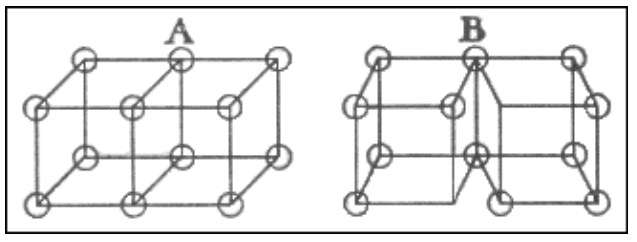
\includegraphics[width=0.6\textwidth]{images/lewis_figure4.png}
	\end{center}
	% Use the following command to remove the colon from the figure label; Always use it within the environment to keep it local
%%%%	\makeatletter \renewcommand{\fnum@figure}[1]{\figurename~\thefigure} \makeatother
	\caption*{Figure 4}

      %  \label{fig:figureX}

%\vspace{-10pt}
\end{figure}

%Fig.4
We may next consider the \emph{double bond} in which four electrons are held conjointly by two atoms.  Thus Figure 4, $A$, may represent the typical structure of the molecule of oxygen.  A characteristic feature of the double bond is its tendency to ''break.''  When this happens in a symmetrical way, as it %insert Fig. 4
will, except in a highly polar environment, it leaves the two atoms concerned in the \emph{odd} state, each with an unpaired electron in the shell.  In so far as a substance with a double bond assumes this other tautomeric form, it will show all the properties of the substances with odd molecules.  Thus Figure 4, $B$, represents this tautomeric form of the oxygen molecule; the equilibrium between forms $A$ and $B$ is entirely analogous to the equilibrium between $\mathrm{N_2O_4}$ and $\mathrm{NO_2}$.  At low temperatures almost every known case of combination with oxygen gives first a peroxide.  This shows that oxygen exists to an appreciable degree in a form which approximates to the form $B$, in which it can add directly to other atoms precisely as ethylene forms addition compounds.  These two forms of oxygen (which, of course, may merge into one another by continuous gradations) can be represented as 
% this makes the atom letters bold:
\renewcommand*\printatom[1]{\ensuremath{\mathbf{#1}}}

% this sets the distance of the Lewis dots from their atom (adjust as desired):
%\setlewis[]{0.3em}{}{}

% this sets the bond distance between atoms (adjust as desired):
%\setatomsep{1.5em}

% this defines a shorthand "dn" so you don't have to keep typing "draw=none"
\tikzset{dn/.style={draw=none}}

\bigskip
\begin{center}
\chemfig{\lewis{0:2:4:,O}} $\;\;$
\chemfig{\lewis{0:2:4:,O}}$\;\;\; \;\textrm{and} \;\;$ 

\bigskip
\chemfig{\lewis{0:2:4:6.,O}} $\;$
\chemfig{\lewis{0:2:6.,O}}$\;\;,$
\end{center}
\bigskip
and the two forms of ethylene\footnote{I shall postpone a discussion of the important bearing of such formulae upon the problem of the conjugate double bond.} as %chemistry

% this makes the atom letters bold:
\renewcommand*\printatom[1]{\ensuremath{\mathbf{#1}}}

% this sets the distance of the Lewis dots from their atom (adjust as desired):
%\setlewis[]{0.3em}{}{}

% this sets the bond distance between atoms (adjust as desired):
%\setatomsep{1.5em}

% this defines a shorthand "dn" so you don't have to keep typing "draw=none"
\tikzset{dn/.style={draw=none}}

\bigskip

\begin{center}
\chemfig{\lewis{0:2:4:,C}
   (-[:90,,,,dn]H)
   (-[:180,,,,dn]H)} $\;\;$
\chemfig{\lewis{0:2:4:,C}
	(-[:0,,,,dn]H)
	(-[:90,,,,dn]H)}$\;\mathrm{and} \;\;$
\bigskip
	\chemfig{\lewis{0:2:4:6.,C}
	   (-[:90,,,,dn]H)
	   (-[:180,,,,dn]H)} $\;$
	\chemfig{\lewis{0:2:6.,C}
		(-[:0,,,,dn]H)
		(-[:90,,,,dn]H)}$\; .$
\end{center}
\bigskip

The instability of multiple bonds and the underlying principle of Baeyer's Strain Theory we shall discuss presently, but before proceeding further in this direction it is important to consider the general relation between the strength of the constraints which hold a molecule together and the stability of the molecule.  The term ''stability'' is used in two very different senses, according as we think of the tendency of a reaction to occur, or the speed of that reaction.  We speak of nitric oxide as an extremely stable substance although it is thermodynamically unstable, and the free energy involved in its decomposition is enormous, but it is so inert that it suffers no appreciable change.  A high degree of inertness means ordinarily very rigid constraints operating within the molecule, but these powerful forces may operate only over a very small distance so that the \emph{work} done in overcoming them them may be very small.  To illustrate this point let us consider a piece of iron suspended by a magnet.  It is drawn downwards by the force of gravity and upwards by the magnetic field, and while the net amount of work obtained by separating it from the magnet and allowing it to fall to earth may be positive, it nevertheless will not fall of itself, but can only be drawn from the magnet by a force far greater than that of gravitation.  So in the case of the molecule, thermodynamic stability is closely associated with the \emph{work} of breaking some bond, but the inertness of the molecule depends upon the \emph{force} required to break that bond.

Before considering triple bonds, for which the cubical structure offers no simple representation, I wish to discuss some ideas in the recent development of which I am greatly indebted to suggestions made by Dr. L. Rosenstein, Dr. E. Q. Adams and Mr. F. R. von Binchowsky, as well as to the work of Mr. A. L. Parson, to which I have already referred.  In my early theory the cube was the fundamental structure of all atomic shells.  We have seen, however, in the case of elements with lower atomic weights than lithium, that the \emph{pair} of electrons forms the stable group, and we may question whether in general the pair rather than the group of eight should not be regarded as the fundamental unit.  Perhaps the chief reasons for assuming the cubical structure were that this is the most symmetrical arrangement of eight electrons, and is the one in which the electrons are farthest apart.  Indeed it seems inherently probable that in elements of large atomic shell (large atomic volume) the electrons are sufficiently far from one another so that Coulomb's law of inverse squares is approximately valid, and in such cases it would seem probable that the mutual repulsion of the eight electrons would force them into the cubical structure.

However, this is precisely the kind of \emph{a priori} reasoning which we have decided not to employ in this paper, and when we consider only known chemical phenomena, and their best interpretation in terms of atomic structure, we are led to assume a somewhat different arrangement of the group of eight electrons, at least in the case of the more nonpolar substances whose molecules are as a rule composed of atoms of small atomic volume.


\begin{figure}
	\begin{center}
		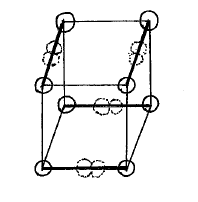
\includegraphics[width=0.3\textwidth]{images/lewis_figure5.png}
	\end{center}
	% Use the following command to remove the colon from the figure label; Always use it within the environment to keep it local
%%%%	\makeatletter \renewcommand{\fnum@figure}[1]{\figurename~\thefigure} \makeatother
	\caption*{Figure 5}

       % \label{fig:figureX}

%\vspace{-10pt}
\end{figure}

%Figure 5

The nature of this arrangement is shown in Figure 5.  The cube representing the electron structure that we have hitherto assumed for the carbon atom is joined to four other atoms, which are not shown in the figure, but which are attached to the carbon atom each by a pair of electrons.  These pairs are indicated by being joined by heavy lines.  Assuming now, at least in such very small atoms as that of carbon, that each pair of electrons has a tendency to be drawn together, perhaps by magnetic force is the magneton theory is correct, or perhaps by other forces which become appreciable at small distances, to occupy positions indicated by the dotted circles, we then have a model which is admirably suited to portray all of the characteristics of the carbon atom.  With the cubical structure it is not only impossible to represent the triple bond, but also to explain the phenomenon of free mobility about a single bond which must always be assumed in stereochemistry.  On the other hand, the group of eight electrons in which the \emph{pairs} are symmetrically paced about the center gives identically the model of the tetrahedral carbon atom which has been of such signal utility throughout the whole of organic chemistry.

As usual, two tetrahedra, attached by one, two or three corners of each, represent respectively the single, the double and the triple bond.  In the first case one pair of electrons is held in common by the two atoms, in the second case two such pairs, in the third case three pairs.

The triple bond represents the highest possible degree of union between two atoms.  Like a double bond it may break one bond, producing two \emph{odd} carbon atoms, but it may also break in a way in which the double bond cannot, to leave a single bond and two carbon atoms (bivalent), each of which has a pair of electrons which is not bound to any other atom.  The three tautomeric forms may be represented in the case of acetylene by 
\bigskip
% this makes the atom letters bold:
\renewcommand*\printatom[1]{\ensuremath{\mathbf{#1}}}

% this sets the distance of the Lewis dots from their atom (adjust as desired):
%\setlewis[]{0.3em}{}{}

% this sets the bond distance between atoms (adjust as desired):
%\setatomsep{1.5em}

% this defines a shorthand "dn" so you don't have to keep typing "draw=none"
\tikzset{dn/.style={draw=none}}
\begin{center}
\chemfig{
	\lewis{0:,H}
	-[:0,,,,dn]\lewis{0:,C}
	-[:0,0.4,,,dn]\lewis{0:,\phantom{C}}
	-[:0,0.4,,,dn]\lewis{0:,\phantom{C}}
	-[:0,,,,dn]\lewis{0:,C}
	-[:0,,,,dn]H
},\phantom{.} \chemfig{
	\lewis{0:,H}
	-[:0,,,,dn]\lewis{0:2.,C}
	-[:0,1.25,,,dn]\lewis{0:2.4:,C}
	-[:0,,,,dn]H
},\phantom{.} and \chemfig{
	\lewis{0:,H}
	-[:0,,,,dn]\lewis{0:2:,C}
	-[:0,,,,dn]\lewis{0:2:,C}
	-[:0,,,,dn]H
}.
\end{center}

\bigskip

\noindent In addition we have a form corresponding to Nef's acetylidene and such forms as may exist in highly polar media, such as the acetylide ion $\mathbf{:C:::C:H}$.

The instability of multiple bonds, as well as the general phenomenon of ring formation in organic compounds is admirably interpreted by the Strain Theory of Baeyer.  This theory may, however, be put into a far more general form if we make the simple assumption that \emph{all atomic kernels repel one another}, and that molecules are held together only by the pairs of electrons which are held jointly by the component atoms.  Thus two carbon atoms with a single bond strive to keep their kernels as far apart as possible, and this condition is met when the adjoining corners of the two tetrahedra lie in the line joining the centers of the tetrahedra.  This is an essential element of Baeyer's theory of ring formation.  When a single bond changes to a multiple bond and the two atomic shells have two pairs of electrons in common, the kernels are forced nearer together and the mutual repulsion of these kernels greatly weakens the constraints at the point of junction.  This diminution in constraint therefore produces a remarkable effect in increasing the mobility of the electrons.  In any part of a carbon chain where a number of consecutive atoms are doubly bound there is in that whole portion of the molecule an extraordinary reactivity and freedom of rearrangement.  This freedom usually terminates at that point in the chain where an atom has only single bonds and in which therefore the electrons are held by more rigid constraints, although it must be observed that an increased mobility of electrons ( and therefore increased polarity) in one part of the molecule always produces some increase in mobility in the neighboring parts.

Let us turn now to a problem in the solution of which the theory which I am presenting shows its greatest serviceability.  The electrochemical theories of Davy and Berzelius were overshadowed by the ''valence'' theory when the attention of chemists was largely drawn to the nonpolar substances of organic chemistry.  Of late the electrochemical theories have come once more into prominence, but there has always been that antagonism between the two views which invariably results when two rival theories are mutually exclusive, while both contain certain element of truth.  Indeed we may now see that with the interpretation which we are now employing the two theories need not be mutually exclusive, but rather complement one another, for the ''valence'' theory, which is the classical basis of structural organic chemistry, deals with the fundamental structure of the molecule, while electrochemical considerations show the influence of positive and negative groups in minor distortions of the fundamental form.  Let us consider once for all that by a negative element or radical we mean one which tends to draw towards itself the electron pairs which constitute the outer shells of all neighboring atoms, and that an electropositive group is one that attracts to a less extent, or repels, these electrons.  In the majority of carbon compounds there is very little of that separation of the charges which gives a compound a polar character, although certain groups, such as hydroxyl, as well as those containing multipole bonds, not only themselves possess a decidedly polar character, but increase, according to principles already discussed, the polar character of all neighboring parts of the molecule.  However, in such molecules as methane and carbon tetrachloride, instead of assuming, as in some current theory, that four electrons have definitely left hydrogen for carbon in the first case, and carbon for chlorine in the second, we shall consider that in methane there is a slight movement of the charges toward the carbon so that the carbon is slightly charged negatively, and that in carbon tetrachloride they are slightly shifted towards the chlorine, leaving the carbon somewhat positive.  We must remember that here also we are dealing with averages and that in a few out of many molecules of methane the hydrogen may be negatively charged and the carbon positively.

In a substance like water the electrons are drawn in from hydrogen to oxygen and we have in the limiting case a certain number of hydrogen atoms which are completely separated as hydrogen ion.  The amount of separation of one of the hydrogen atoms, and therefore the degree of ionization, will change very greatly when the other hydrogen atom is substituted by a positive or negative group.  As a familiar example we may consider acetic acid, in which one hydrogen is replaced by chlorine, $\mathrm{H_2ClCCOOH}$.  The electrons, being drawn toward the chlorine, permit the pair of electrons joining the methyl and carboxyl groups to approach nearer to the methyl carbon.  This pair of electrons, exercising therefore a smaller repulsion upon the other electrons of the hydroxyl oxygen, permit these also to shift in the same direction.  In other words, all the electrons move toward the left, producing a greater separation of the electrons from the hydrogen of the hydroxyl, and thus a stronger acid.  This simple explanation is applicable to a vast number of individual cases.  It need only be borne in mind that although the effect of such a displacement of electrons at one end of a chain proceeds throughout the whole chain it becomes less marked the greater the distance,\footnote{The distance to be considered is the \emph{actual} distance.  Thus when a chain of five or six links assumes a ring-like form, the two ends have a great influence upon each other, as has been pointed out by Michael in numerous cases.} and the more rigid the constraints which hold the electrons in the intervening atoms.

This brief account of the theory of atomic and molecular structure could be extended almost indefinitely by illustrations of its application to numerous types of compounds, but I believe enough has been said to show how, through simple hypotheses, we may explain the most diverse types of chemical union and how we may construct models which illustrate the continuous transition between the most polar and the most nonpolar of substances.  I shall therefore conclude this paper with a brief discussion of a phenomenon which bears closely upon the ideas which have been presented here.

\section*{The Color of Chemical Compounds.}

When a particle is held in position by definite constraints, it is capable of vibrating with a definite frequency, and this frequency is determined solely by the magnitude of the constraints\footnote{If the constraints are not uniform in all directions there will in general be three fundamental frequencies corresponding to the three axes of constraint, along which the constraints are respectively at a maximum, at a minimum and at a minimax.} and by the mass of the particle.  When such a particle is electrically charged and subjected to the alternating electromagnetic forces which constitute a beam of light, and when the frequency of the light is near to the characteristic frequency of the particle, the latter is set to vibrating and through frictional processes the energy of the light is absorbed.

The two kinds of charged particles which exist in chemical substances are charged atoms and electrons.  The former, on account of their relatively large mass, have low characteristic frequencies which are, as far as I am aware, always far below the frequencies of visible light and therefore cause absorption only in the ultra-red [infrared] spectrum.  The electrons, on the other hand, because of their small mass and the rigid constraints by which they are ordinarily bound, usually have frequencies higher than those of visible light and therefore absorb light only in the ultraviolet.  The majority of substances therefore show no special absorption of visible light and are therefore colorless.

When, however, either by a change in the constitution of the molecule or through a change in the environment, the constraints acting upon an electron become weaker, the frequency of that electron becomes less.  It may then begin to absorb visible light of the highest frequency, namely violet and blue, and the transmitted light is therefore yellow.  Whenever a colorless substance becomes colored through slight changes by substitution of somewhat different groups within the molecule, or by gradual change in the environment, the substance is always \emph{yellow}.  But if the changes are made more pronounced and the characteristic frequency of the electron or electrons concerned is still further lowered, so that the maximum of absorption is in some other part of the visible spectrum, different colors will be produced, and ultimately when the electron is nearly freed from constraint, as in the case of an alkali metal dissolved in liquid ammonia, the maximum of absorption is in the ultra-red [infrared] and red, and a blue color results.

Now colored substances are the very ones in which, according to our theory, the electrons are least firmly held.  Thus such substances as nitrogen dioxide and sodium vapor, which contain an uneven number of electrons and which therefore hold one of the electrons very loosely, are colored.  If, however, sodium combines with chlorine the electron becomes firmly held by the latter element and when nitrogen dioxide combines even with itself to form $\mathrm{N_2O_4}$ the electron is again firmly held and the color disappears.  Indeed, with the exception of $\mathrm{NO}$, every one of the substances with odd molecules which we have listed is colored.  The tri-aryl methyls show a remarkable analogy to $\mathrm{NO_2}$.  In nonpolar media they show an increase of color when the conditions so change as to increase the amount of the monomolecular or odd molecules.  Thus the color is increased by rising temperature or by increasing dilution, but the color of these substances in a polar environment is due to another cause, the discussion of which would lead us into the whole question of the triphenyl methane dyes.

Turning now to substances containing an even number of electrons, we see in the case of the halogens how the intensity and character of the color vary with the polar character.  Thus the electrons which are concerned in the union of the two atoms of iodine are held by weaker constraints than in the case of bromine, and so on through the group. The electrons in fluorine, being most firmly held, absorb only the extreme violet end of the visible spectrum.

In general, color and a high degree of polarity go hand in hand, as is abundantly shown in the great class of organic dyes.  Both of these phenomena are due to the same cause, namely the weakness of the constraints acting upon one or more electrons.

It has frequently been noticed that there is a striking parallelism between color and the possibility of tautomeric change, and it has been assumed by some that color is in some way due to an alternation between two extreme tautomeric forms.  But this is not precisely the case.  When electrons are sufficiently free to produce absorption in the visible spectrum, that part of the molecule in which they are will always be highly polar and reactive, and there will be opportunity for free transition from one limiting form to another.  Thus if a tautomeric process consists chiefly in the movement of electrons, there will be electrons in some molecules which are hung by loose constraints between the two extreme forms, and these are the electrons which will have a sufficiently low characteristic frequency to produce color.

In the class of elements which have not been considered in the present paper many are found, such as manganese and cobalt, which give a great variety of colored compounds.  The difficulty in interpreting the compounds of these elements in terms of the present theory lies, I believe, in the fact that the kernel of the atom is not uniquely and permanently defined.  It seems probable that in these elements there is a possibility of the transfer of electrons either from one part of the kernel to another, or between the kernel and the outer shell, or possibly between two separate outer shells of the same atom, and that electrons which are suspended midway between two such stages are responsible for the absorption of light in these cases. \vspace{5 mm}

BERKELEY, CAL.


\newpage

\section*{Glossary of Chemical Terms for Lewis}

Chemical structures are given with lines representing one single bond each, so that a pair of parallel lines represents a double bond.  In general, bonds to hydrogens are not drawn, for simplicity. 

\begin{itemize}


\item[]{\textbf{Acetic acid:} the formula is $\mathrm{H_3COOH}$.  When one of the hydrogens on the left-most carbon (the methyl group) is replaced by a chlorine, the electrons tend to shift in that direction.  See images below:}



\begin{figure}[h]
\vspace{-15pt}
\begin{center}
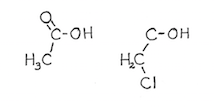
\includegraphics[width=0.4\textwidth]{images/lewis_notefig1.png}
\end{center}
%\vspace{-10pt}
%\caption{}
\vspace{-30pt}
\end{figure}



\item[]{\textbf{Acetylene, acetylidene, acetylide ion:} the prefix ``acetyl'' is used for a chemical substance when a carbon is triple bonded to another carbon.}	
	
\item[]{\textbf{Alcohol:} a general term for a substance in which a carbon group is attached to a hydroxyl group.  Ethyl alcohol, the active ingredient in alcoholic beverages, is shown below:}

\begin{figure}[h]
\vspace{-15pt}
\begin{center}
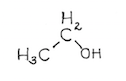
\includegraphics[width=0.2\textwidth]{images/lewis_notefig2a.png}
\end{center}
%\vspace{-10pt}
%\caption{}
\vspace{-30pt}
\end{figure}


\item[]{\textbf{Alkali metal:} any element on the periodic table in the Lithium column.}

\item[]{\textbf{Amine:} a general germ for a substance in which a nitrogen atom is bound to one or more carbon groups.}

\item[]{\textbf{Ammonia:} a small molecule in which one nitrogen is bound to 3 hydrogens.}

\item[]{\textbf{Aryl:} a general term for a chemical substance with a benzene-like ring that is bound to something besides hydrogen.  For example, phenol is shown below:}

\begin{figure}[h]
\vspace{-15pt}
\begin{center}
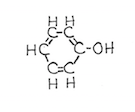
\includegraphics[width=0.2\textwidth]{images/lewis_notefig3.png}
\end{center}
%\vspace{-10pt}
%\caption{}
\vspace{-30pt}
\end{figure}


\item[]{\textbf{Benzene:} a nonpolar chemical formed from 6 carbons connected in a hexagonal ring, with hydrogens on the carbons.  A two-dimensional structure is given below:}

\begin{figure}[h]
\vspace{-15pt}
\begin{center}
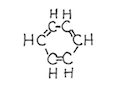
\includegraphics[width=0.2\textwidth]{images/lewis_notefig4.png}
\end{center}
%\vspace{-10pt}
%\caption{}
\vspace{-30pt}
\end{figure}


\item[]{\textbf{Carboxyl group:} a carbon with a double bond to one oxygen and a single bond to a hydroxyl group.}

\item[]{\textbf{Chlorides, hypochlorites, chlorites, chlorates, perchlorates:} chlorine compounds with successively more oxygens bound.  Chlorides have no oxygen (e.g.\ sodium chloride, or table salt).  Hypochlorites have one oxygen bound to the chlorine (e.g.\ bleach), chlorites have 2 oxygens, chlorates have 3, and perchlorates have 4 oxygens bound to the chloride ion.}

\item[]{\textbf{Electrophile:} a chemical substance that tends to attract electrons from other chemical substances.}

\item[]{\textbf{Electropositive:} used of a substance when it has a tendency to repel electrons.}

\item[]{\textbf{Ester:} a general term for a chemical substance in which an oxygen is bound by two carbon groups, but one of those carbon groups has another oxygen bound with a double bond.  Esters tend to have a strong odor.  Se the image below for allyl hexanoate, which is largely responsible for the color of pineapples (source: Wikipedia):}


\begin{figure}[h]
\vspace{-15pt}
\begin{center}
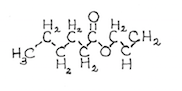
\includegraphics[width=0.4\textwidth]{images/lewis_notefig6.png}
\end{center}
%\vspace{-10pt}
%\caption{}
\vspace{-30pt}
\end{figure}


\item[]{\textbf{Ether:} a general term for a chemical substance in which oxygen is bound to two carbon groups.  The simplest ether, dimethyl ether, is shown below.}

\begin{figure}[h]
\vspace{-10pt}
\begin{center}
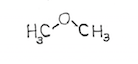
\includegraphics[width=0.3\textwidth]{images/lewis_notefig5.png}
\end{center}
%\vspace{-10pt}
%\caption{}
\vspace{-30pt}
\end{figure}

\item[]{\textbf{Ethylene:} a small molecule with two carbons double bonded to each other.  The structure is shown below:}

\begin{figure}[h]
\vspace{-15pt}
\begin{center}
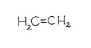
\includegraphics[width=0.3\textwidth]{images/lewis_notefig6a.png}
\end{center}
%\vspace{-10pt}
%\caption{}
\vspace{-30pt}
\end{figure}


\item[]{\textbf{Halogen:} any element on the periodic table in the Fluorine column.}


\item[]{\textbf{Hexane:} a nonpolar chemical framed from 6 carbons arranged linearly with 14 hydrogens (total) attached to the carbons.}

\begin{figure}[h]
\vspace{-10pt}
\begin{center}
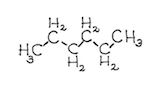
\includegraphics[width=0.3\textwidth]{images/lewis_notefig7.png}
\end{center}
%\vspace{-10pt}
%\caption{}
\vspace{-30pt}
\end{figure}


\item[]{\textbf{Inorganic:} chemical substances that arise independent of living organisms, including, but not limited to minerals, salts, acids, and alkalis.}

\item[]{\textbf{Isomer:} a chemical substance composed of the same number and kinds of atoms as another chemical, but with a different molecular structure.}

\item[]{\textbf{Ketone:} a general term for a chemical substance with a carbon chain that has one of the carbons in the middle bound with a double bond to oxygen.  See structure below:}

\begin{figure}[h]
\vspace{-15pt}
\begin{center}
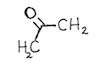
\includegraphics[width=0.2\textwidth]{images/lewis_notefig8.png}
\end{center}
%\vspace{-10pt}
%\caption{}
\vspace{-30pt}
\end{figure}


\item[]{\textbf{Methyl group:} a carbon bound with three hydrogens that is attached to something.}

\item[]{\textbf{Nonpolar:} a chemical substance is considered ``nonpolar'' if it gives no evidence that there is any separation of charge.}

\item[]{\textbf{Nt:} Lewis refers to ``Niton,'' which was later renamed ``Radon.''}

\item[]{\textbf{Organic:} chemical substances that arise due to the action of a living organism.  The term ``organic'' came to mean nearly any complex molecule containing carbon.}

\item[]{\textbf{Peroxide:} a chemical substance that contains two oxygen molecules with a single bond between them.  Hydrogen peroxide is shown below:}

\begin{figure}[h]
\vspace{-15pt}
\begin{center}
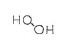
\includegraphics[width=0.2\textwidth]{images/lewis_notefig8a.png}
\end{center}
%\vspace{-10pt}
%\caption{}
\vspace{-30pt}
\end{figure}


\item[]{\textbf{Polar:} a chemical substance is considered ``polar'' if it gives evidence of being a dipole, that is, if it seems that one part of the molecule is charged slightly positive and another slightly negative.}

\item[]{\textbf{Tautomerism:} occurs when two or more forms of a molecule can interconvert easily.  An example is given below.}

\begin{figure}[h]
\vspace{-10pt}
\begin{center}
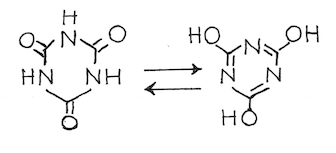
\includegraphics[width=0.4\textwidth]{images/lewis_notefig9.png}
\end{center}
%\vspace{-10pt}
%\caption{}
\vspace{-30pt}
\end{figure}


\item[]{\textbf{Valence:} a term that refers to the chemical combining power of lan element.  For example, if a particular element can combine with 2 hydrogens, it has a valence of 2.}


\newpage

\begin{figure}[h]
\vspace{10pt}
\begin{center}
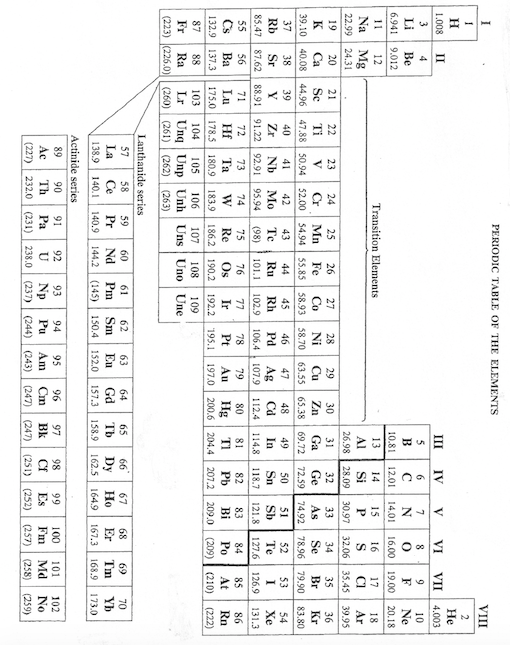
\includegraphics[width=1.0\textwidth]{images/lewis_periodictable.png}
\end{center}
%\vspace{-10pt}
%\caption{}
%\vspace{-30pt}
\end{figure}

\end{itemize}


\end{document}


%%% Local Variables:
%%% mode: latex
%%% TeX-master: t
%%% End:
